%
 Let $3x+2y=6$ intersects the x-axis and y-axis at $\vec{A}$ and $\vec{B}$ respectively.
\begin{enumerate}
\item Let $\vec{A}$ = $\myvec{x\\0}$
\begin{align}
3x = 6
\\
\implies x=2
\\
\vec{A} = \myvec{2\\0}
\end{align}
\item Let $\vec{B}$ = $\myvec{0\\y}$ 
\begin{align}
2y = 6
\\
\implies y=3
\\
\vec{B} = \myvec{0\\3}
\end{align}
\item Origin = $\myvec{0\\0}$ does not satisfy the equation $3x+2y<6$. \\
$\implies$ The solution is the right side of the line $3x+2y=6$ \\

\item The following python code is the diagrammatic representation of the solution in Fig.\ref{fig:3.11.6_line_ineq}
\begin{lstlisting}
solutions/6/codes/linear_inequalities/linear_inequalities.py
\end{lstlisting}

\begin{figure}[!ht]
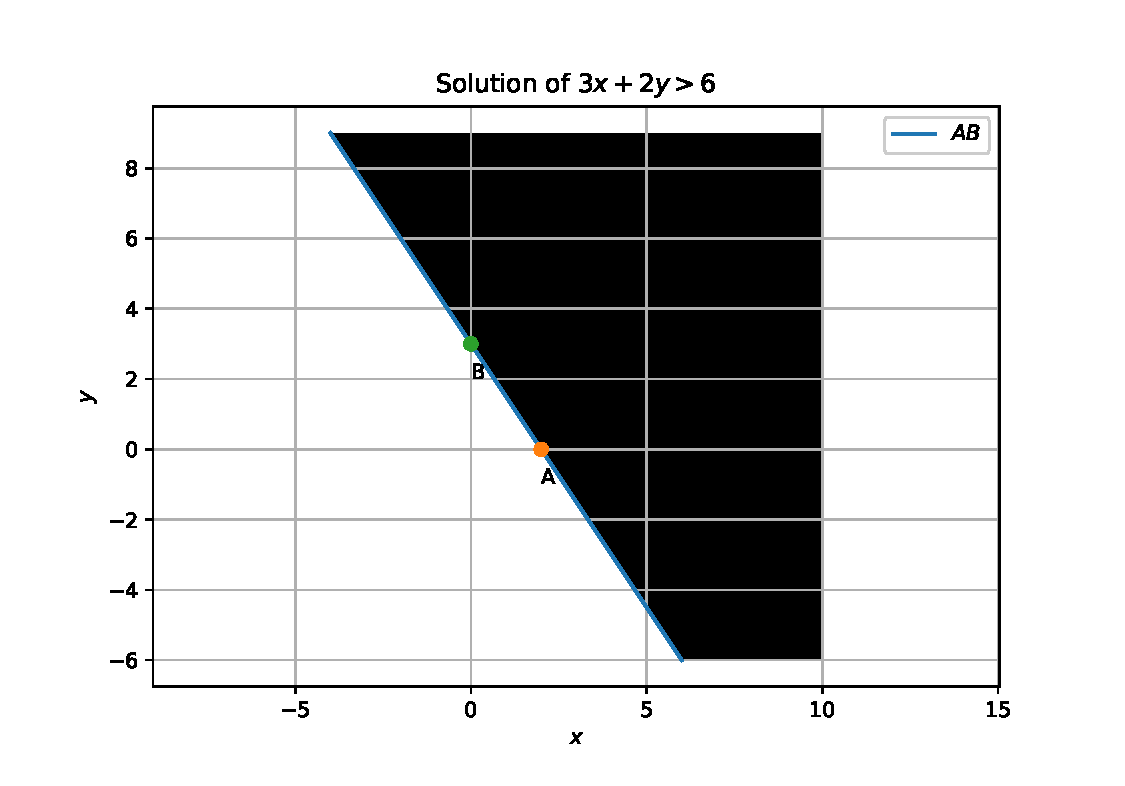
\includegraphics[width=\columnwidth]{./solutions/6/codes/line/linear_inequalities/linear_inequalities.eps}
\caption{}
\label{fig:3.11.6_line_ineq}
\end{figure} 

\end{enumerate}
 

 
 
